\chapter{Handwritten Text Detection using PEMAN based CNN architecture}

In earlier studies, we trained a model for the handwritten dataset but it was only an ANN. This time we use a CNN based approach which is known to be more efficient in image processing tasks.

The dataset used is the MNIST dataset. The MNIST dataset is a large database of handwritten digits that is commonly used for training various image processing systems. The MNIST database contains 60,000 training images and 10,000 testing images. The images are grayscale, 28x28 pixels. The neural network has 784 input neurons and 10 output neurons. The output neurons are the digits from 0 to 9. The neural network has 2 hidden layers with one being a convolutional layer and one being a linear layer. The convolutional layer has 10 input channels and 20 output channels. The linear layer has 320 neurons.

Upon training with 8 bits accuracy, the accuracy of the model came out to be 98.80\%. This shows that even with reduced bit accuracy from PEMAN, simply using CNN boosted the accuracy over even non-quantized version of the linear model. 

\section{Optimization}

As we peer into this study, we can see that in many of the multiplication operations, we are using the same weights for different inputs, as there is only one kernel for the entire image, that is, one entire time cycle. This means that for an entire time cycle, one phase shifter can remain constant. This improves the requirement and the hardware complexity by a significant amount.

For more detailed study, the weights of non-quantized version and the quantized version were compared. This comparison needed to be done to gain insights to which of the weights were more affected by the quantization that others. The weight errors were plotted in a heatmap to see the distribution of the errors. The heatmap is shown in figure \ref{weightdist}.

\begin{figure}
	\centering
	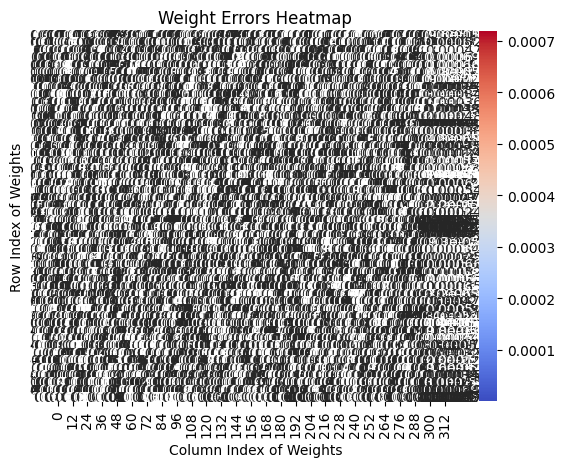
\includegraphics[width=\textwidth]{images/weightdist.png}
	\caption{Distribution of weights}
	\label{weightdist}
\end{figure}

As we can see from the heatmap, the weight error distribution is actually very random. This means that the quantization error is not concentrated on any particular weight. This is a good sign as it means that the quanization does not affect any particular types of features of weights and can be used for any kind of weights.